\begin{frame}{The first wave of BCI: control your world}
  \begin{columns}[c,onlytextwidth]
    \column{.61\textwidth}
      \small
      \NTXPoint{Consumer headsets opened the door}{Games, feedback, and device-control experiments made brain signals something people could explore outside a lab.}
      \NTXPoint{The promise brought people together}{Hardware to try, software to write, and results to compare: a starting point for hacknights and community building.}
      {\small\textbf{Early entry points}\par}
      {\small Muse \enspace EMOTIV \enspace NeuroSky \enspace OpenBCI\par}
      \medskip
      {\small\textbf{The ecosystem kept growing}\par}
      {\small Neurosity \enspace BrainBit \enspace Bitbrain \enspace MindAffect\par}
    \column{.35\textwidth}
      \centering
      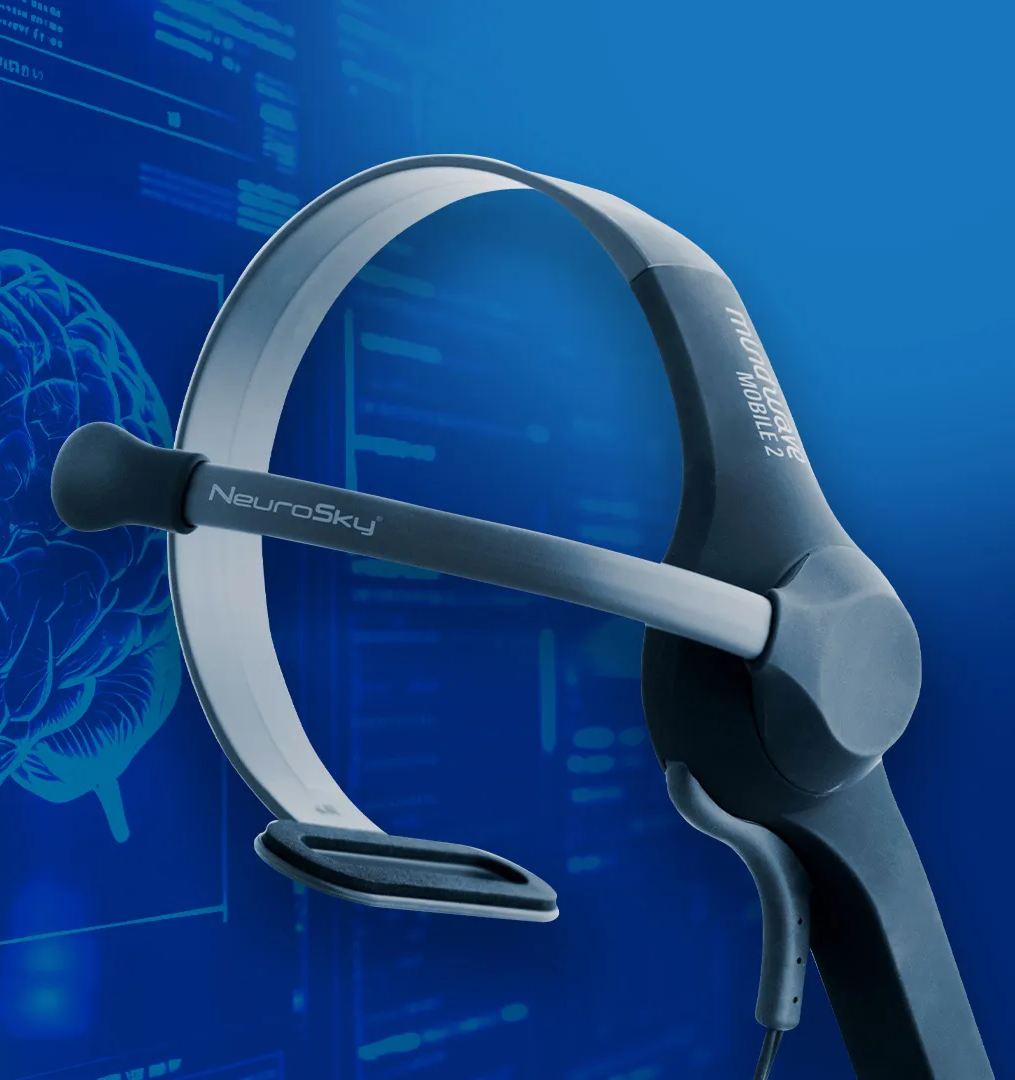
\includegraphics[width=\linewidth,height=40mm,keepaspectratio]{assets/history/neurosky-mindwave-mobile2.png}\par\smallskip
      {\tiny NeuroSky MindWave Mobile 2\newline Later model illustrating the headset lineage\newline Photo: NeuroSky\par}
  \end{columns}
  {\tiny\color{NTXMuted}Morgan's community-history framing. Sources: \href{https://www.emotiv.com/blog/how-emotiv-epoc-changed-the-world-of-neurotechnology}{EMOTIV}; \href{https://choosemuse.com/pages/team}{Muse}; \href{https://neurosky.com/neurosky-products/mindwave-headset/}{NeuroSky}; \href{https://openbci.com/community/openbci-on-kickstarter/}{OpenBCI}\par}
  \note{[05:30--07:00] Morgan's first wave means consumer and accessible non-invasive BCI driving community development, not the invention of BCI. The promise attracted people; making hardware work and understanding signals gave them a reason to learn together. Early milestones: EPOC in 2009, NeuroSky games and developer tools, OpenBCI's 2013 Kickstarter, and Muse's 2014 meditation-feedback launch. Muse was not primarily marketed for external device control. Neurosity, BrainBit, Bitbrain, and MindAffect represent the expanding ecosystem, not simultaneous launches or equal roles in NTX's founding. These span consumer products, open hardware, research devices, and BCI software, not interchangeable headsets. The MindWave Mobile 2 image depicts a later model. Control your world is an aspiration, not unrestricted thought reading, universal control, or clinical efficacy. No vendor sponsorship or formal partnership is implied. Transition to the chapter map. Detailed sources and boundaries: assets/history/first-wave-bci-sources.md.}
\end{frame}
